\documentclass[a4paper,11pt]{article}
\usepackage{/home/rweye/Nextcloud/Documents/Overleaf/Styles/Cours}
%\usepackage{typearea}
%\usepackage[utf8]{inputenc}
%\usepackage[T1]{fontenc}
\usepackage{color}
\usepackage{mwe}
\usepackage{listings}    
\usepackage{etoolbox}    

\definecolor{mygreen}{rgb}{0,0.6,0}
\definecolor{mygray}{rgb}{0.47,0.47,0.33}
\definecolor{myorange}{rgb}{0.8,0.4,0}
\definecolor{mywhite}{rgb}{0.98,0.98,0.98}
\definecolor{myblue}{rgb}{0.01,0.61,0.98}

\newcommand*{\FormatDigit}[1]{\ttfamily\textcolor{mygreen}{#1}}
%% https://tex.stackexchange.com/questions/32174/listings-package-how-can-i-format-all-numbers
\lstdefinestyle{FormattedNumber}{%
    literate=*{0}{{\FormatDigit{0}}}{1}%
             {1}{{\FormatDigit{1}}}{1}%
             {2}{{\FormatDigit{2}}}{1}%
             {3}{{\FormatDigit{3}}}{1}%
             {4}{{\FormatDigit{4}}}{1}%
             {5}{{\FormatDigit{5}}}{1}%
             {6}{{\FormatDigit{6}}}{1}%
             {7}{{\FormatDigit{7}}}{1}%
             {8}{{\FormatDigit{8}}}{1}%
             {9}{{\FormatDigit{9}}}{1}%
             {.0}{{\FormatDigit{.0}}}{2}% Following is to ensure that only periods
             {.1}{{\FormatDigit{.1}}}{2}% followed by a digit are changed.
             {.2}{{\FormatDigit{.2}}}{2}%
             {.3}{{\FormatDigit{.3}}}{2}%
             {.4}{{\FormatDigit{.4}}}{2}%
             {.5}{{\FormatDigit{.5}}}{2}%
             {.6}{{\FormatDigit{.6}}}{2}%
             {.7}{{\FormatDigit{.7}}}{2}%
             {.8}{{\FormatDigit{.8}}}{2}%
             {.9}{{\FormatDigit{.9}}}{2}%
             %{,}{{\FormatDigit{,}}{1}% depends if you want the "," in color
             {\ }{{ }}{1}% handle the space
             ,%
}


\lstset{%
  backgroundcolor=\color{mywhite},   
  basicstyle=\footnotesize,       
  breakatwhitespace=false,         
  breaklines=true,                 
  captionpos=b,                   
  commentstyle=\color{red},    
  deletekeywords={...},           
  escapeinside={\%*}{*)},          
  extendedchars=true,              
  frame=shadowbox,                    
  keepspaces=true,                 
  keywordstyle=\color{myorange},       
  language=Octave,                
  morekeywords={*,...},            
  numbers=left,                    
  numbersep=5pt,                   
  numberstyle=\tiny\color{mygray}, 
  rulecolor=\color{black},         
  rulesepcolor=\color{myblue},
  showspaces=false,                
  showstringspaces=false,          
  showtabs=false,                  
  stepnumber=2,                    
  stringstyle=\color{myorange},    
  tabsize=2,                       
  title=\lstname,
  emphstyle=\bfseries\color{blue},%  style for emph={} 
}    

%% language specific settings:
\lstdefinestyle{Arduino}{%
    style=FormattedNumber,
    keywords={void},%                 define keywords
    morecomment=[l]{//},%             treat // as comments
    morecomment=[s]{/*}{*/},%         define /* ... */ comments
    emph={HIGH, OUTPUT, LOW},%        keywords to emphasize
}

\newtoggle{InString}{}% Keep track of if we are within a string
\togglefalse{InString}% Assume not initally in string


\newcommand{\chnum}{Chapitre 17}
\newcommand{\chtitle}{Caractérisation d'un circuit et d'un dipôle}
\newcommand{\dtype}{TP}

\begin{document}

\maketitle
La photorésistance est un capteur utilisé pour détecter l'allumage des lumières lorsque la luminosité diminue dans une habitation ou dans l'espace public. \emph{Comment contrôler un éclairage avec une photorésistance ?}

\begin{figure}[h]
	\caption{\textbf{La photodiode}}
	Module photodiode ou capteur de lumière compatible Grove permettant de détecter la présence de lumière. Ce module se raccorde sur une entrée analogique du Base Shield via un câble quatre connecteur fourni.\\
	Une photodiode est un composant semi-conducteur ayant la capacité de capteur un rayonnement du domaine optique et de le transformer en signal électrique (la tension de crête est à \SI{540}{nm}). Un rayonnement lumineux sur la photodiode favorise le passage du courant à polarisation inverse.\\
La résistance du capteur diminue alors au fur et à mesure que l'intensité lumineuse augmente. La tension de sortie analogique varie selon l'intensité lumineuse mesurée.
\begin{center}
		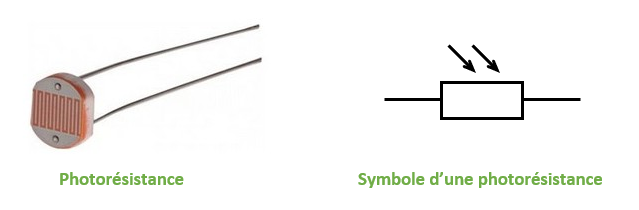
\includegraphics[width=.3\linewidth]{Ressources/Photoresistance.png}
	\end{center}
\end{figure}

\begin{figure}[h!]
	\caption{\textbf{Le dispositif avec microcontrôleur (Arduino) et photocapteur}}
	La tension $U_E$ aux bornes du module photodiode est envoyée sur l'entrée $A_0$ (entrée analogique) du microcontrôleur. Un programme téléversé dans le microcontrôleur, est exécuté en permanence. Il contrôle la tension $U_S$ qui vaut \SI{0}{V} à \SI{5}{V}, selon la valeur de $U_E$, celle-ci variant avec l'éclairement capté par la photodiode. La tension $U_S$ au niveau de la sortie $D2$ (entré ou sortie numérique) alimente un circuit d'éclairage composé d'une DEL et de sa résistance de protection.
	\begin{center}
		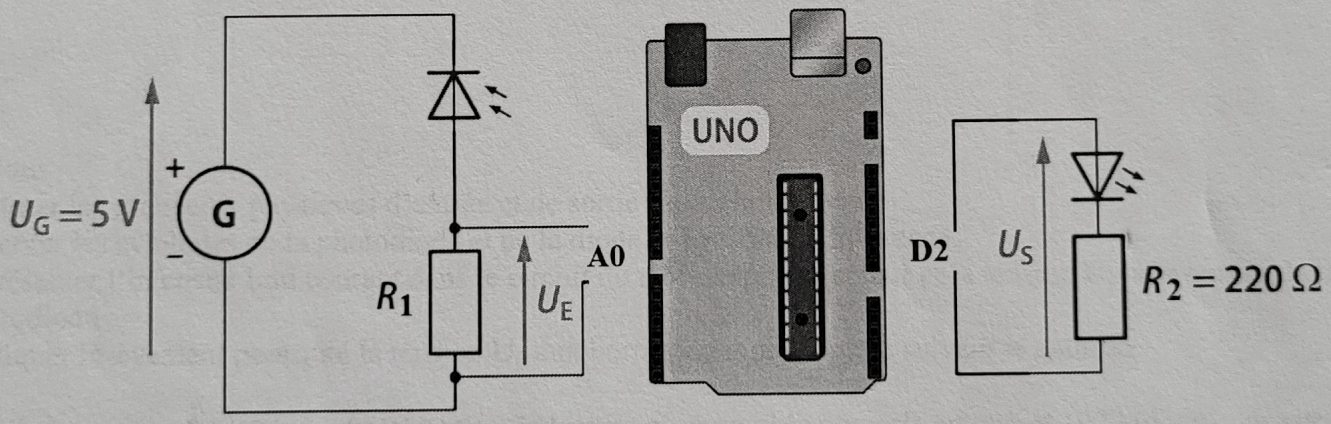
\includegraphics[width=.5\linewidth]{Ressources/ArduinoEclairage.png}
	\end{center}
	\label{fig2}
\end{figure}

\begin{figure}[h!]
	\caption{Lancement du programme}
	\begin{minipage}{.7\linewidth}
	\begin{lstlisting}[style=Arduino]
//commande d'un eclairage

const int photoD = A0 ; //branchement module photoDiode
const int DELPin = 2 ; //branchement module DEL
float N ; // niveau lu
float UE ; // tension d'entree

// int ValeurSeuil = ...... ;

void setup() {
    Serial.begin(9600) ;
    pinMode(photoD, INPUT) ;
    pinMode(DELPin, OUTPUT) ;
}

void loop(){
    N = analogRead(photoD) ; // lecture sur le module photoD
    // float UE = ...... ; // calcul de la tension d'entree

    delay(1000) ;
    Serial.print(N) ;
    Serial.print("  tension d'entree UE = ");
    //Serial.print(UE);
    Serial.println("V");
}
\end{lstlisting}
	\end{minipage}
	\begin{minipage}{.3\linewidth}
	\begin{itemize}
		\item Ouvrir le programme
		\item Cliquer sur "outil"
		\item Cliquer sur "Port"
		\item Sélectionner le COM Arduino Uno
		\item Vérifier la syntaxe du programme et corriger les erreurs
		\item Cliquer sur "Téléverser"
		\item Le programme s'exécute automatiquement
	\end{itemize}
	\end{minipage}
\end{figure}

\begin{figure}[h!]
	\textbf{Questions :}
	\begin{enumerate}
	\item Nommer les grandeurs physiques d'entrée et de sortie de la photodiode.
	\item Observer les symboles de la photodiode et de la diode et justifier la différence. (Doc.fig2)
	\item Représenter l'intensité $I$ du courant dans le circuit du module photocapteur et la tension $U_p$ aux bornes de la photodiode.
	\item Exprimer brièvement pourquoi la tension $U_E$ aux bornes du module varie suivant le courant.
\end{enumerate}
La fonction \emph{analogRead(photoD)} permet la lecture d'un nombre compris entre 0 et 1023 (donc codé sur 10 bits),  \textbf{proportionnel} à la tension mesurée sur l'entrée analogique : 0 correspond à \SI{0}{V} et 1023 correspond à \SI{5}{V}.

\begin{enumerate}[resume]
	\item Nommer la variable dans laquelle est stockée la valeur lue sur l'entrée analogique.
	\item Déterminer le calcul nécessaire pour obtenir $U_E$ à partir de cette variable et afficher le résultat. Compléter le programme et le téléverser à nouveau.
	\item Déterminer une valeur seuil en Volt qui déclenche l'allumage d'une DEL lorsque la luminosité est trop faible.
	\item Ajouter des instructions conditionnelles pour :
	\begin{itemize}
		\item allumer les réverbères lorsque la lumière est faible et afficher un message
		\item éteindre les réverbères dans le cas contraire et afficher un message également
	\end{itemize}
\end{enumerate}

\begin{multicols}{2}
\textbf{Instructions pour l'alimentation de la DEL :}
\begin{lstlisting}[style=Arduino]
	digitalWrite(DELPin, LOW) ; // Allumage
	digitalWrite(DELPin, HIGH) ; // Extinction
\end{lstlisting}

\columnbreak
\textbf{Écriture d'un test conditionnel} :
\begin{lstlisting}[style=Arduino]
if (condition) {
	bloc d'instructions ;
}
else {
	bloc d'instructions ;
}
\end{lstlisting}
\end{multicols}
\end{figure}
\end{document}